\subsection{Data Analysis}
Our first step in analyzing the collected data was to plot it. Since the shape of the energy spectrum is given by the derivative of the I-V curve, it was necessary to numerically calculate the derivative. The method we chose to do this was to fit a linear function to $n$ neighboring data points using a straightforward least squares approach. The slope of the fitted function was taken as the derivative.This had the additional benefit of performing some smoothing. Of course there is some information lost in the process, but this was not deemed critical as the number of points collected was generally much larger than $n$.

In order to estimate the energy gap of our Pb sample it was necessary to evaluate the integral in \ref{ins_numerical}, 
\begin{eqnarray*}\label{ins_numerical2}
I^{NS} &=& \frac{C^{NN}}{e} \int_{0}^{\infty} dx\ \frac{x+\Delta}{\sqrt{x(x+2 \Delta)}} \times
		\nonumber \\
		&\times& [f(x+ \Delta-eV)-f(x+ \Delta +eV)],
		\nonumber \\
\end{eqnarray*}
and compare the results to the experimental data. In order to do so we split the integral in 2 parts. The high energies were evaluated numerically using a Romberg-Method algorithm \cite{recipes}, while the lower energies were estimated analytically. It was assumed that $ [f(x+ \Delta-eV)-f(x+ \Delta +eV)] \approx \text{const.}$ for small $x$, as it is finite and nonzero for $x=0$, while the other part, $\frac{x+\Delta}{\sqrt{x(x+2 \Delta)}}$, diverges for $x\to0$. It can, however, be integrated analytically up to $0$, thus enabling us to efficiently integrate for all $x$. 
\begin{equation*}\label{num}
 \int_{0}^{a} dx\ \frac{x+\Delta}{\sqrt{x(x+2 \Delta)}} = \sqrt{a(2\Delta+a)}
\end{equation*}

To get the conductance curve, the resulting theoretical I-V curve was derivated in the same manner as the experimental data, i.e. with the same degree of smoothing, to ensure their comparability.

\begin{figure}[h!]
\centering
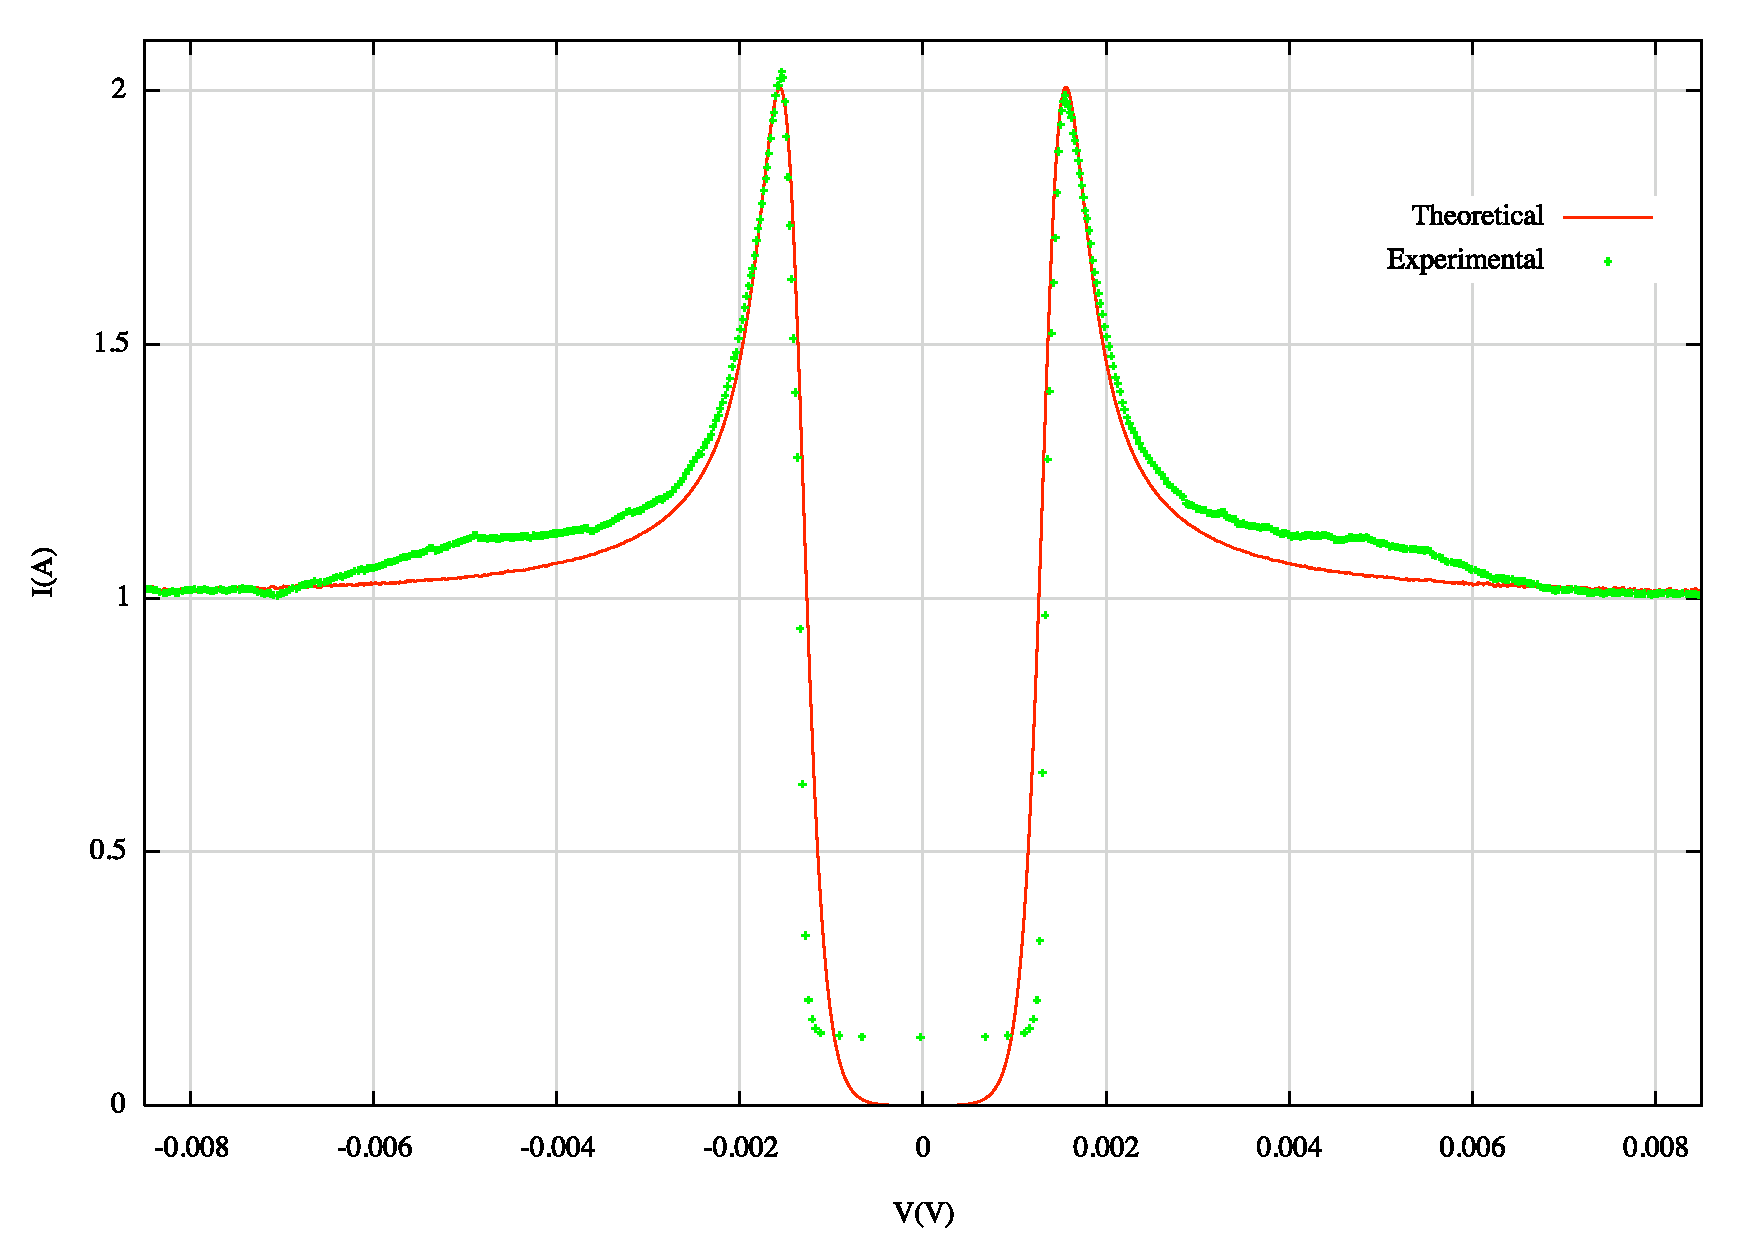
\includegraphics[width=0.45\textwidth]{gv_theo_exp_7}
\caption{\small Experimental data and BCS theoretical prediction for $1.45 K$. The different density of states of Pb with respect to BCS causes the discrepancy. 
\label{gv_theo_exp_7}}
\end{figure}

%1.- BCS does not fully describe the measured data. The density of states is different... --> Residual
When plotting the derivatives in this way and comparing them qualitatively to each other for some arbitrary but reasonable values of $T$,$\Delta$ and $C_{NN}$ it quickly becomes apparent that there are certain qualitative differences between the experimental results and the results predicted by the BCS theory. Specifically, there are some bulges in the conductance curves outside the gap in the experimental data which are not present in the theory (see fig. \ref{gv_theo_exp_7}).

\begin{figure}[h!]
\centering
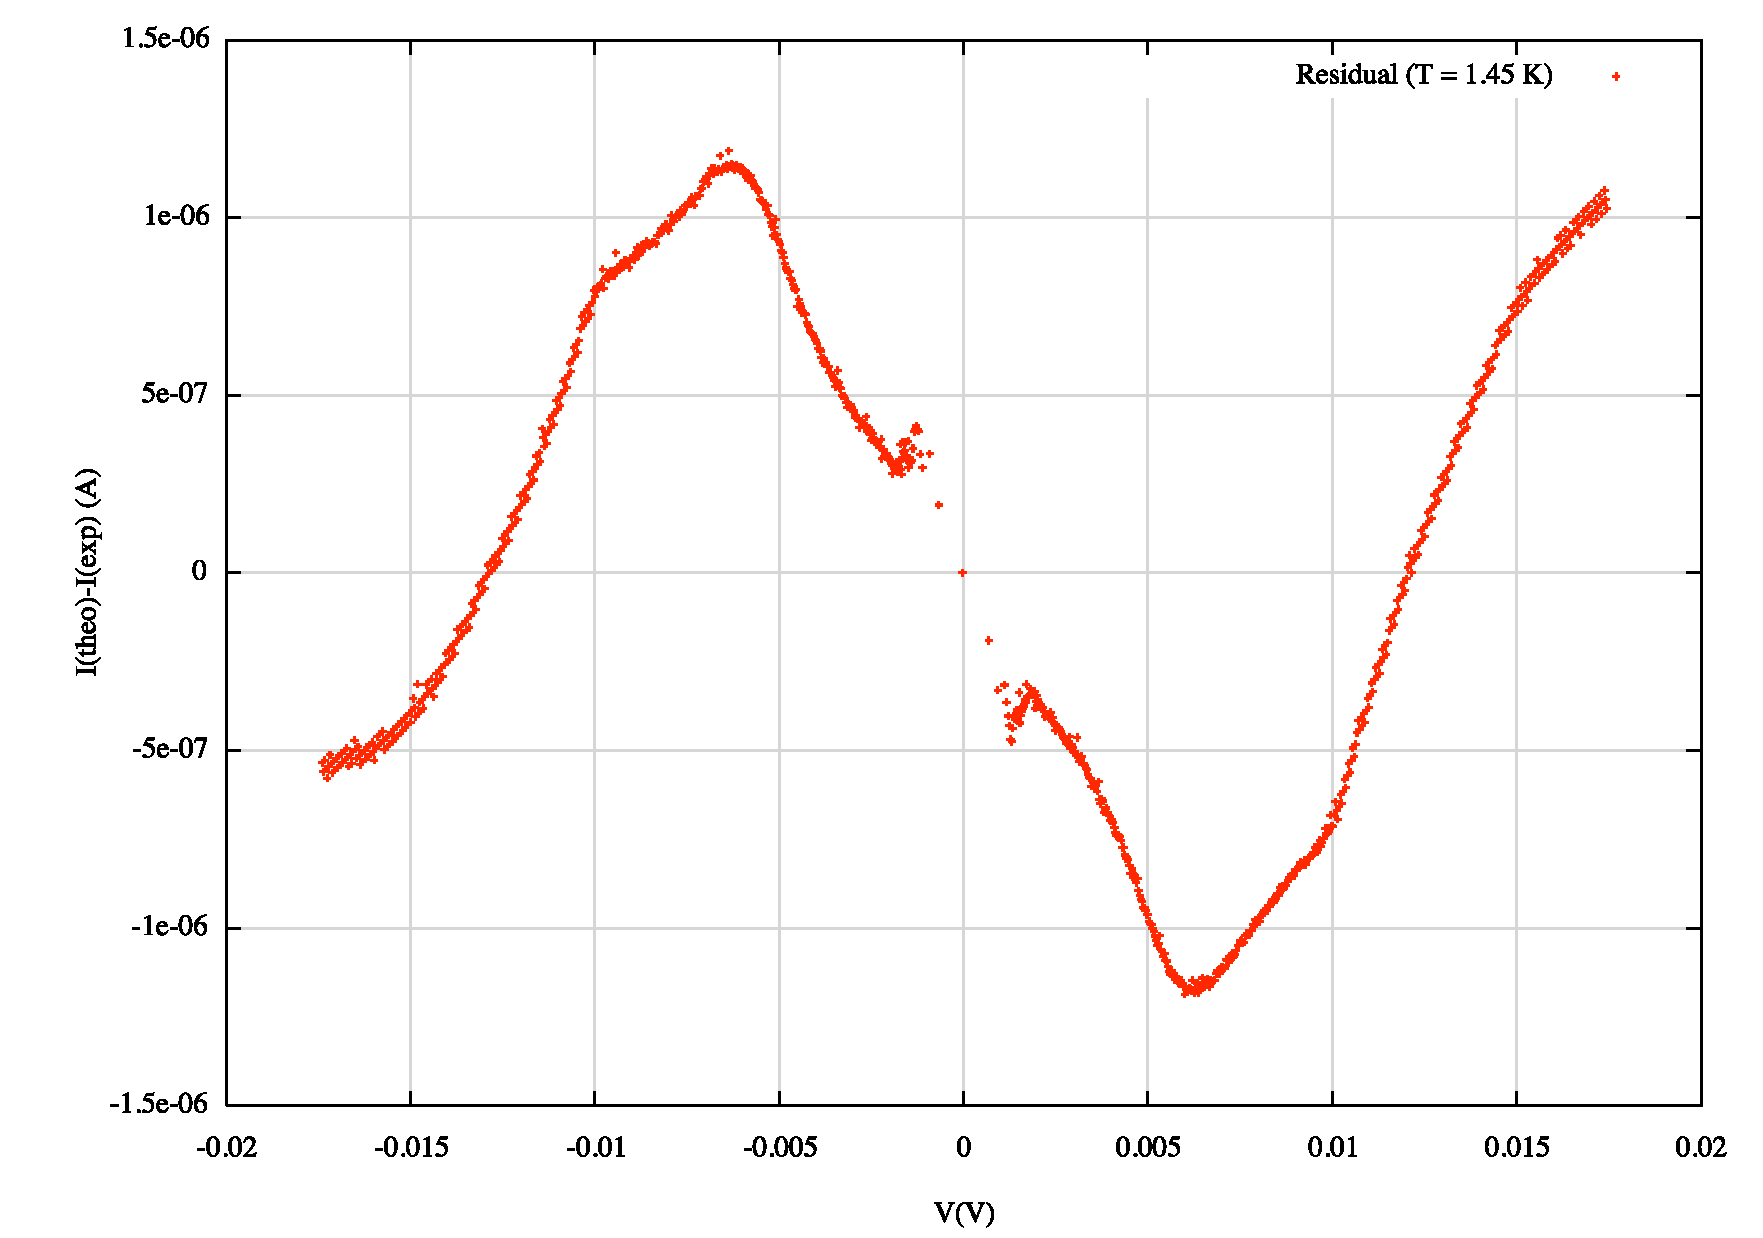
\includegraphics[width=0.45\textwidth]{residual}
\caption{\small Residual between theoretical and experimental current curve for $1.45 K$. The phonon structure arises clearly. 
\label{residual}}
\end{figure}


Our best guess as to what might be causing this effect is electron-phonon scattering. It seems not to vary significantly with Temperature (see fig. \ref{gv_3-4-5-7}) in the range of our observations. The shape of the deviation from the current predicted by BCS theory can be seen in figure \ref{residual}. Giaver also reports the same effect in a later paper \cite{giaever2}, and suggests it can be accounted for using a non-constant energy-gap parameter.

The initial idea for estimating the energy gap and the other parameters of the model($T$,$C_{NN}$) was to fit them using a least squares method. We tried to do so using a Levenberg-Marquard routine. This approach proved inefficient, with the results being rather dependent on the initial guess, and convergence reached at unexpected values. This is probably due to the algorithm over-fitting in the region affected by the model insufficiencies described above, as well as the high degree of nonlinearity exhibited by the function.

A more feasible method was to estimate normal-normal conductance and temperature from other measurements, and then fitting the value of the gap "by hand".

\begin{figure}[h!]
\centering
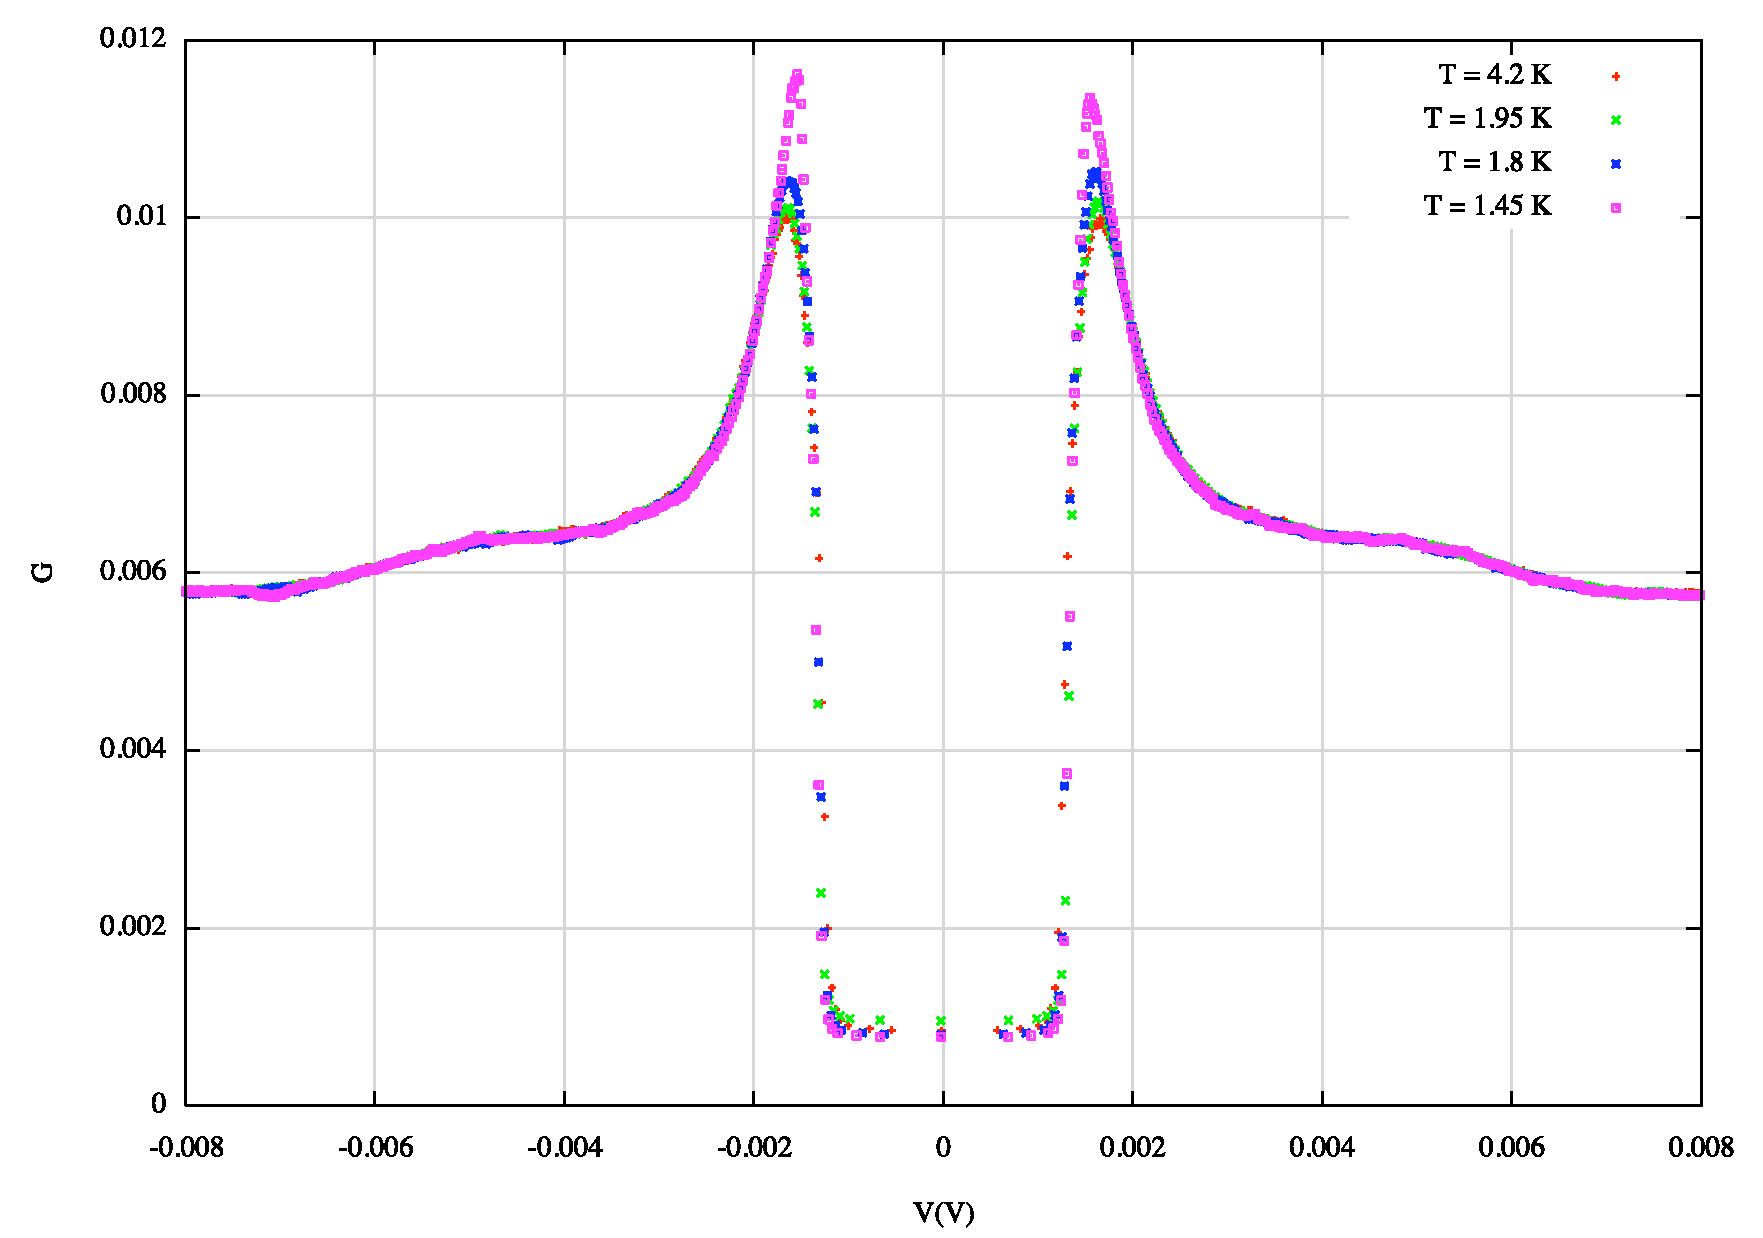
\includegraphics[width=0.45\textwidth]{gv_3-4-5-7}
\caption{\small Measured conductance for 4 different temperatures. The peaks coincidence sustains the nearly invariance of the gap for this temperature range. The phonon structure is the same for all.
\label{gv_3-4-5-7}}
\end{figure}


\subsection{Results}

\begin{figure}[h!]
\centering
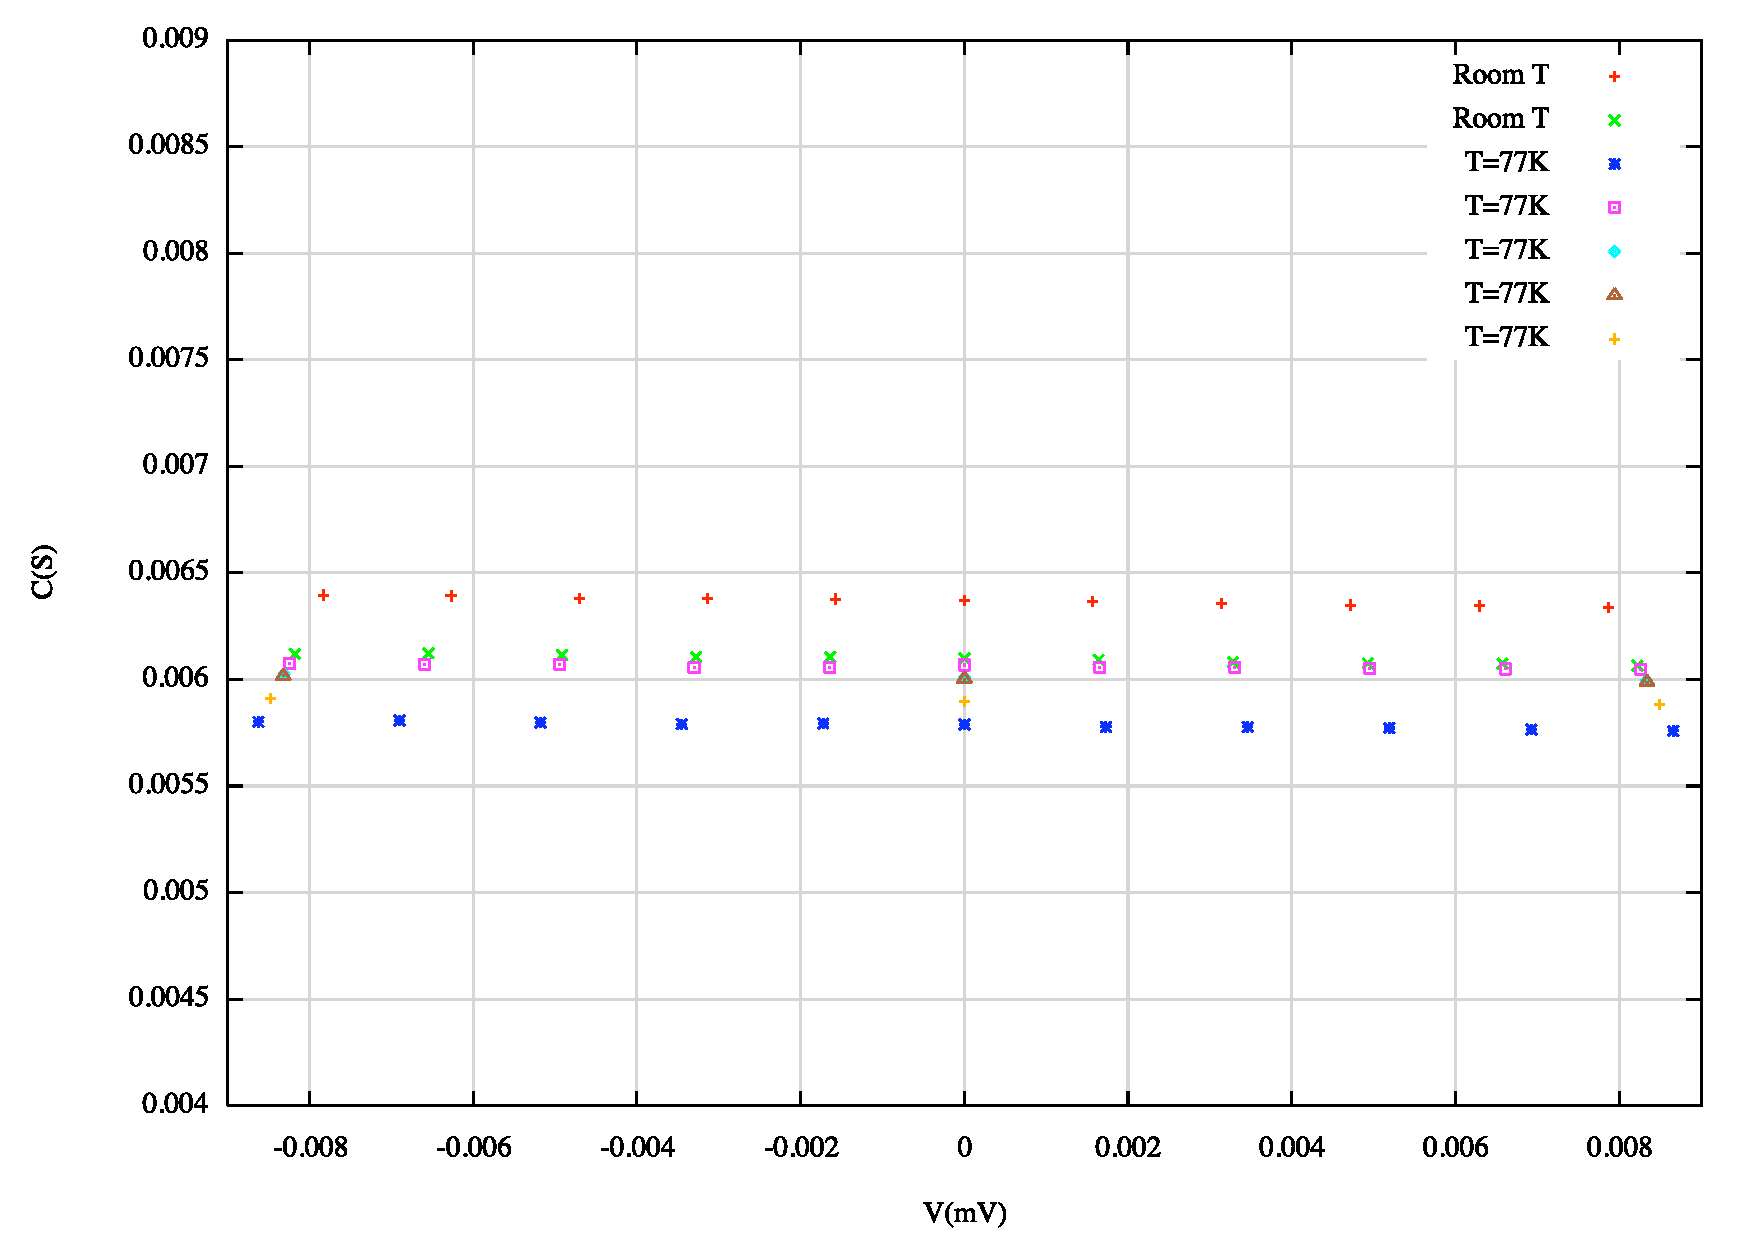
\includegraphics[width=0.45\textwidth]{conductance2}
\caption{\small Conductance curves . \label{conductance2}}
\end{figure}

Prior to inserting He into the cryostat as described, we measured the conductivity of the sample several times at different temperatures. From these measurements we determined $C_{NN}=0.006\pm0.0005 S$. The values taken in the relevant range of voltages can be seen in  fig. \ref{conductance2}.

%	2nd : T by helium vapor pressure --> manometer�?�? error??? 
The values for the Temperature were obviously different for each measurement. We determined it by means of associating temperatures to pressures at the surface of the $He^4$ using the vapor pressure curve. As described earlier, there was a manometer connected to the cryostat, and readings were taken at every measurement. This assumes that the pressure is the same at the surface and at the top of the cryostat, where the measurement is taken \ednote{Why is this assumption OK}. The measurements from the manometer might also have been faulty, the pressure shown at room pressure was too low (700 mbar). The difference caused by this miscalibration seemed to be very low at lower pressures, of about 5 mbar, and hence less than $0.1\ K$.

\begin{figure}[h!]
\centering
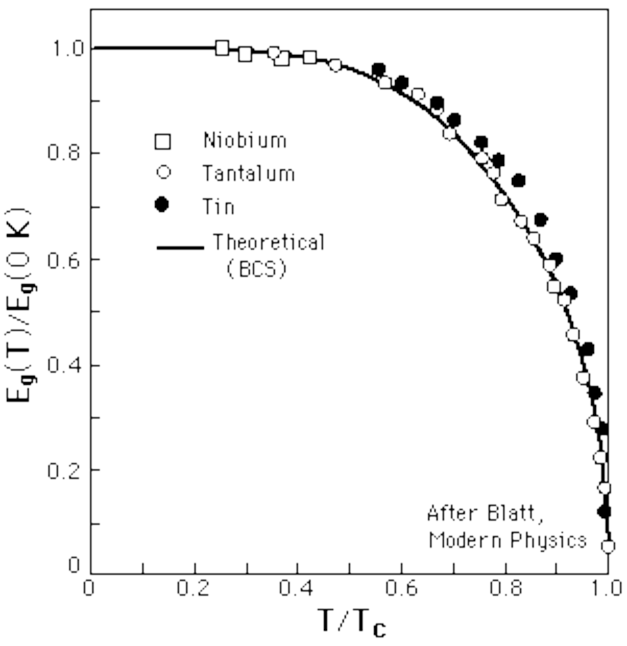
\includegraphics[width=0.45\textwidth]{bcs_gap2}
\caption{\small Reduced values of the observed energy gap as a function of the reduced temperature, after Towsend and Sutton. The solid curve is drawn for the BCS theory. \label{bcs_gap2}}
\end{figure}

With the other parameters now fixed, the with of the energy gap can now be fitted. Theoretically it depends on the temperature, but in the range of temperatures we measured in this change is very small, as can be seen in figure \ref{bcs_gap2}. The amount of change for temperatures between $1.2\ K$ and $4.2\ K$ is $\approx 0.07\Delta_0$, which is about $0.1 meV$, the error we expected to be caused by our fitting of the value "by hand", and we consequently assumed the value to be the same in all the measurements. Fitting the width by this process for the different measurements gave us a value of  $1.4\pm0.1$ meV. The error is a rough estimate based on the finesse with which we manually adjusted the gap. It is probably a little to large, yet we decided to give this slightly higher figure to account for the uncertainties in the temperature.

\begin{figure}[h!]
\centering
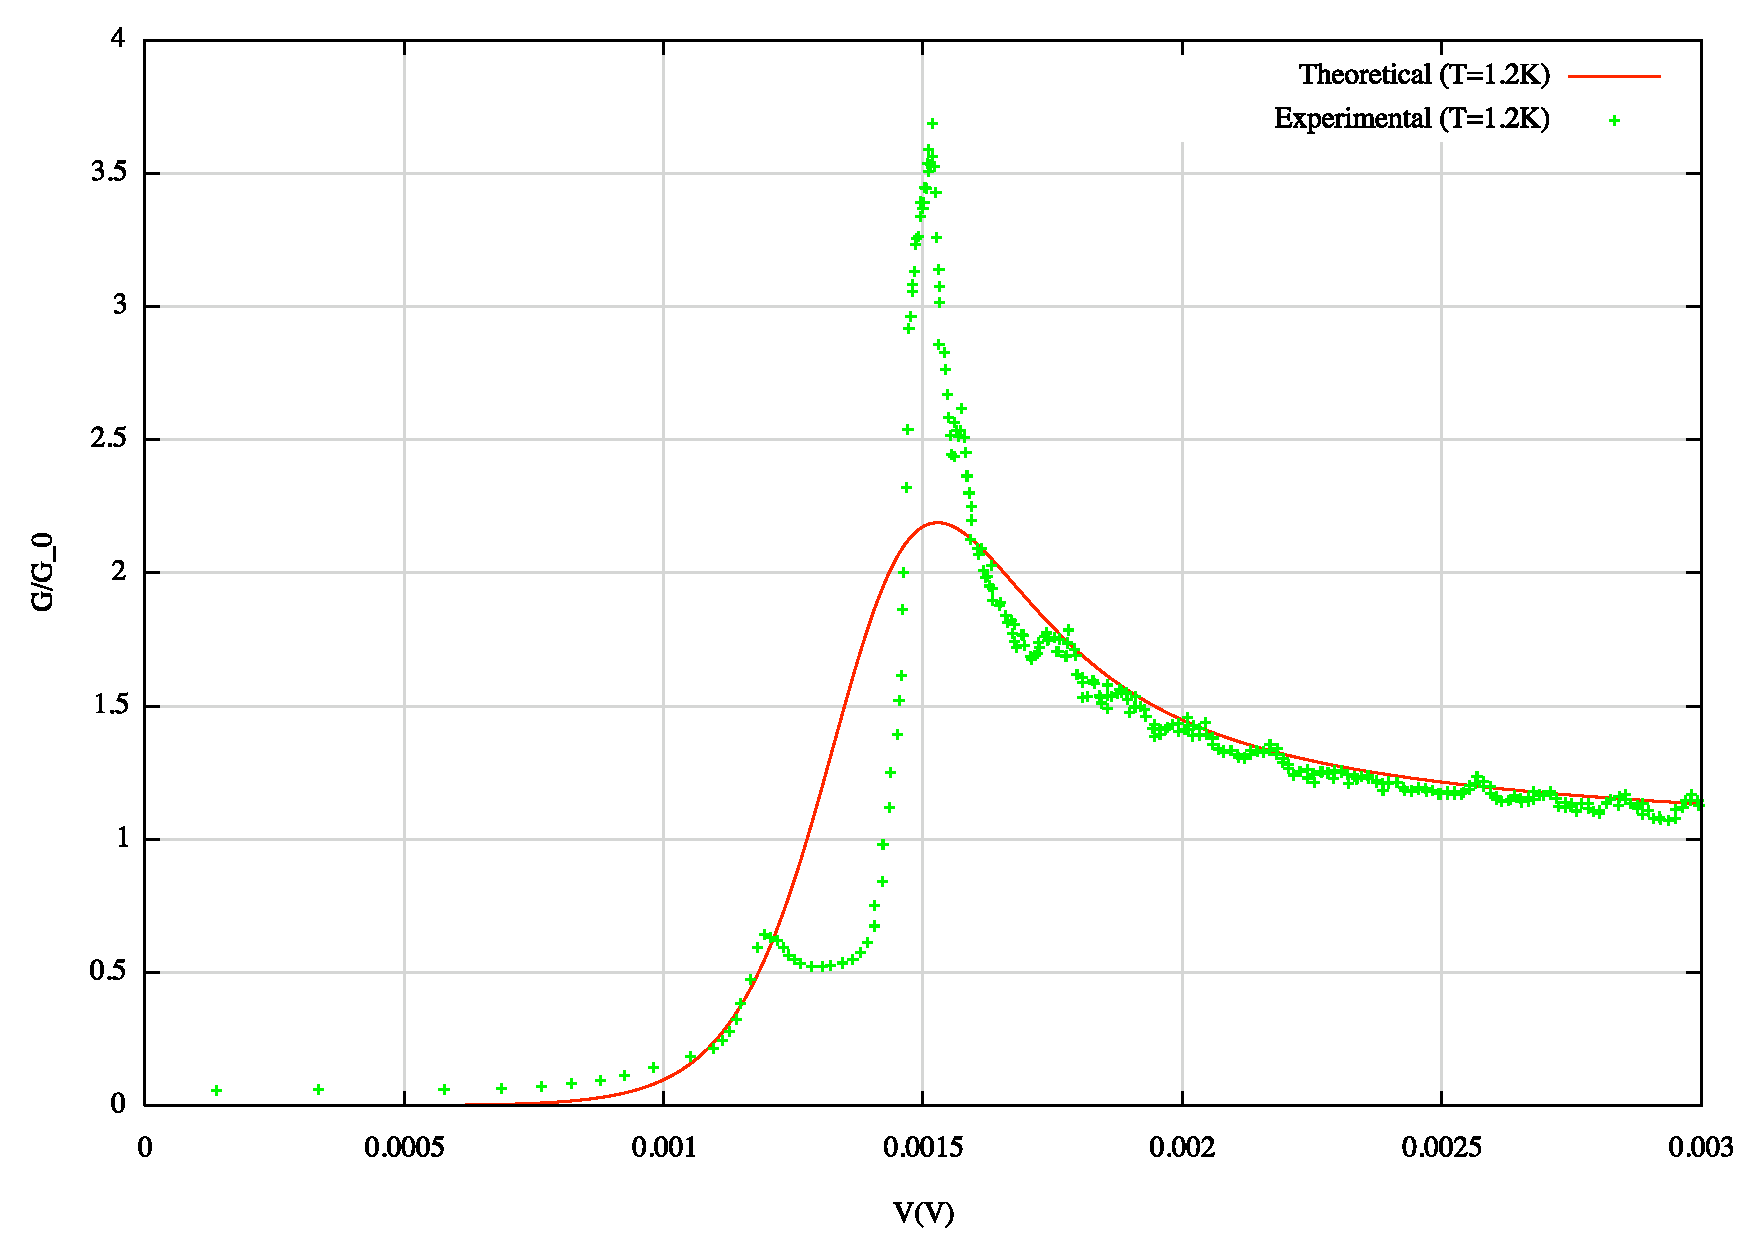
\includegraphics[width=0.45\textwidth]{gv_theo_exp_10}
\caption{\small Experimental data and BCS theoretical prediction for $1.2 K$. There is a second peak due to the superconductor transition of some parts of the Aluminum.
\label{gv_theo_exp_10}}
\end{figure}

The measurement at the lowest temperature we could perform gives qualitatively different results. In fig. \ref{gv_theo_exp_10} can be seen the appearance of new effects. The transition temperature $T_c$ for Aluminum is $1.140 K$, and we have established experimentally the temperature for data as $1.2 K$. However, due to the difference between bulk properties and those that we must consider here for thin films, the $T_c$ is a little bit greater (see \cite{films}).

The situation is qualitatively clear now, i.e. the temperature has fallen enough to let some portions of Aluminum change to superconducting state, creating this combined effect between normal-superconductor and superconductor-superconductor junctions. It can be explained by considering a sum of junctions of these two kinds in parallel, so as to produce an I-V curve with peaks inside the gap of the Aluminum. For a superconductor-superconductor junction appear two peaks, located at $| \Delta_1-\Delta_2|$ and $(\Delta_1+\Delta_2)$.



